% !TeX root = cm1015-cm-notes.tex

\documentclass{article}
\usepackage[utf8]{inputenc}
\usepackage[english]{babel}
\usepackage{xcolor}

\usepackage{minted}
\setminted{fontfamily=tt}
% Disable italics for comments and configure color of code block text
\usepackage{etoolbox}
\BeforeBeginEnvironment{minted}{\def\FancyVerbFormatLine{\def\baselinestretch{1}\small\color{white}}}
\AtBeginEnvironment{minted}{\let\itshape\relax}

\usepackage{graphicx}
\usepackage{tikz}

\usepackage[scaled]{helvet}
\renewcommand*\familydefault{\sfdefault}

\usepackage[hmargin=2.54cm, vmargin=2.54cm]{geometry}

% Define custom color
\definecolor{darkgray}{RGB}{13, 17, 23}
\definecolor{lightgrey}{RGB}{216, 222, 233}

\pagecolor{darkgray}
\color{lightgrey}

\begin{document}

\begin{titlepage}
    \centering
    \vspace*{2cm}
    
    {\LARGE\bfseries CM1015 - Computational Mathematics}\\[0.8cm]
    {\large\bfseries BSc Computer Science}\\[0.5cm] 
    {\large\textnormal{Nathan Donovan}}\\[1.5cm] 

    
\includegraphics[scale=0.1]{../images/university-of-london-logo.png}\\[1.5cm] 
    {\Large\bfseries University of London}\\[1cm]
    {\large April 2024}

    \vfill
    
\end{titlepage}

\newpage
\section*{Number Bases}
\subsection*{Decimal}

\noindent Number bases relate to the amount of digits used to represent a number. 
The decimal system is base 10, meaning it uses 10 digits (0-9) to represent numbers. 
The value of a number is calculated by multiplying each digit by the base raised to the power of its position. 
For example, the number 123 in decimal is calculated as follows:

\vspace{0.5cm}

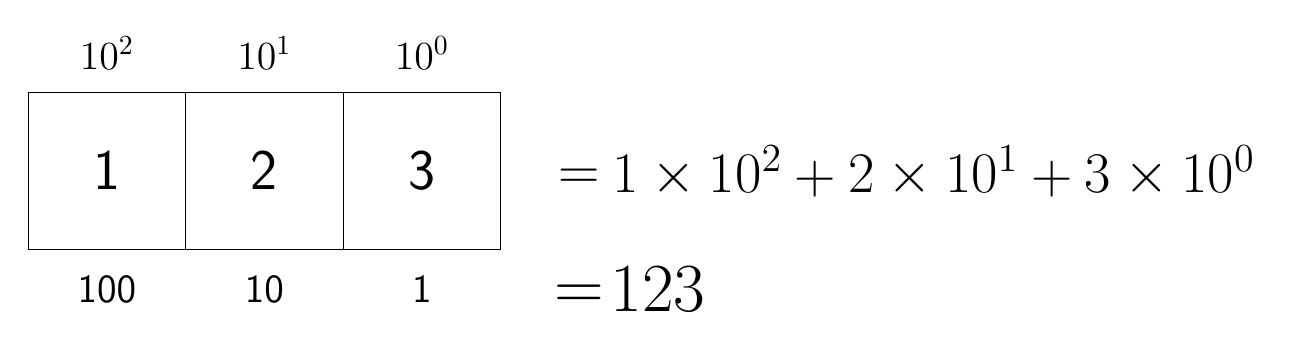
\begin{tikzpicture}
    \foreach \x/\y/\base/\dec in {0/1/2/100, 2/2/1/10, 4/3/0/1} {
        % Base value above the square
        \node at (\x,2.5) {\Large$10^{\base}$};
        % Draw the larger square
        \draw (\x-1,0) rectangle ++(2,2);
        % Number inside the square
        \node at (\x,1) {\huge \y};
        % Decimal value below the square
        \node at (\x,-0.5) {\Large\dec};
    }
    \node at (6,0.9) {\huge $=$};
    \node at (7.5,1) {\huge $1 \times 10^2$};
    \node at (9,0.9) {\huge $+$};
    \node at (10.5,1) {\huge $2 \times 10^1$};
    \node at (12,0.9) {\huge $+$};
    \node at (13.5,1) {\huge $3 \times 10^0$};

    \node at (6,-0.6) {\Huge $=$};
    \node at (7,-0.5) {\Huge $123$};
\end{tikzpicture}

\vspace*{0.5cm}

\subsection*{Binary}

\noindent The binary system is base 2, meaning it uses 2 digits (0-1) to represent numbers. Binary numbers are calculated in the same way as decimal numbers, but using powers of 2 instead of 10. For example, the binary number 101 in decimal is calculated as follows:

\vspace*{0.5cm}

\begin{tikzpicture}
    \foreach \x/\y/\base/\dec in {0/1/2/4, 2/0/1/2, 4/1/0/1} {
        % Base value above the square
        \node at (\x,2.5) {\Large$2^{\base}$};
        % Draw the larger square
        \draw (\x-1,0) rectangle ++(2,2);
        % Number inside the square
        \node at (\x,1) {\huge \y};
        % Decimal value below the square
        \node at (\x,-0.5) {\Large\dec};
    }
    \node at (6,0.9) {\huge $=$};
    \node at (7.5,1) {\huge $1 \times 2^2$};
    \node at (9,0.9) {\huge $+$};
    \node at (10.5,1) {\huge $0 \times 2^1$};
    \node at (12,0.9) {\huge $+$};
    \node at (13.5,1) {\huge $1 \times 2^0$};

    \node at (6,-0.6) {\Huge $=$};
    \node at (7,-0.5) {\Huge $5$};
\end{tikzpicture}

\vspace*{0.5cm}

\subsection*{Hexadecimal}

\noindent The hexadecimal system is base 16, meaning it uses 16 digits (0-9, A-F) to represent numbers. Hexadecimal numbers are calculated in the same way as decimal numbers, but using powers of 16 instead of 10. For example, the hexadecimal number 1A3 in decimal is calculated as follows:

\vspace*{0.5cm}

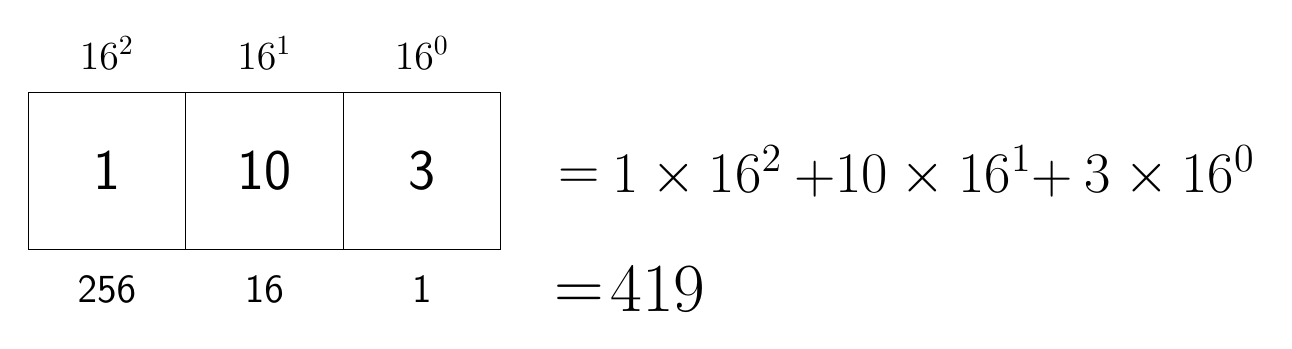
\begin{tikzpicture}
    \foreach \x/\y/\base/\dec in {0/1/2/256, 2/10/1/16, 4/3/0/1} {
        % Base value above the square
        \node at (\x,2.5) {\Large$16^{\base}$};
        % Draw the larger square
        \draw (\x-1,0) rectangle ++(2,2);
        % Number inside the square
        \node at (\x,1) {\huge \y};
        % Decimal value below the square
        \node at (\x,-0.5) {\Large\dec};
    }
    \node at (6,0.9) {\huge $=$};
    \node at (7.5,1) {\huge $1 \times 16^2$};
    \node at (9,0.9) {\huge $+$};
    \node at (10.5,1) {\huge $10 \times 16^1$};
    \node at (12,0.9) {\huge $+$};
    \node at (13.5,1) {\huge $3 \times 16^0$};

    \node at (6,-0.6) {\Huge $=$};
    \node at (7,-0.5) {\Huge $419$};
\end{tikzpicture}

\newpage

\subsection*{Generic Base Conversion to Decimal}

\noindent To convert any base to decimal, the following method can be used:

\begin{enumerate}
    \item Write the number in the base you are converting from.
    \item Multiply each digit by the base raised to the power of its position.
    \item Add the results together to get the decimal value.
\end{enumerate}

\vspace*{0.25cm}

\noindent Formula: $d_n \times b^n + d_{n-1} \times b^{n-1} + \ldots + d_1 \times b^1 + d_0 \times b^0$

\vspace*{0.25cm}

\noindent Where: $d_n$ is the digit at position $n$, $b$ is the base, and $n$ is the position of the digit.

\vspace*{0.25cm}

\noindent Example, shown with above symbols:

\vspace*{0.5cm}

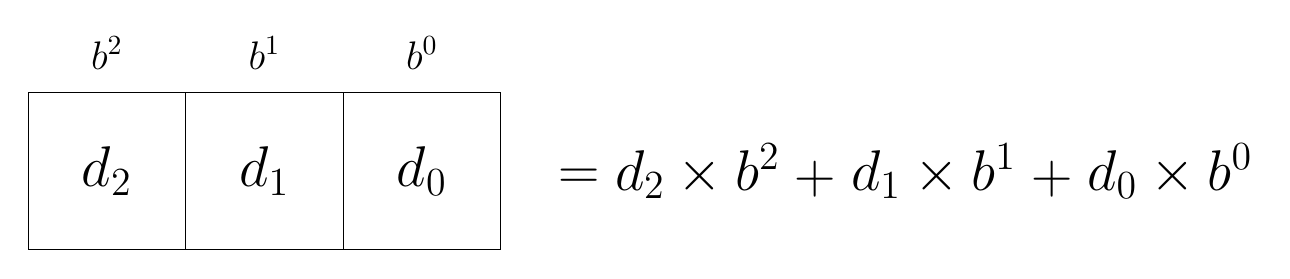
\begin{tikzpicture}
    \foreach \x/\y/\base/\dec in {0/1/2/4, 2/0/1/2, 4/1/0/1} {
        % Base value above the square
        \node at (\x,2.5) {\Large$b^{\base}$};
        % Draw the larger square
        \draw (\x-1,0) rectangle ++(2,2);
        % Number inside the square
        \node at (\x,1) {\huge $d_{\base}$};
    }
    \node at (6,0.9) {\huge $=$};
    \node at (7.5,1) {\huge $d_2 \times b^2$};
    \node at (9,0.9) {\huge $+$};
    \node at (10.5,1) {\huge $d_1 \times b^1$};
    \node at (12,0.9) {\huge $+$};
    \node at (13.5,1) {\huge $d_0 \times b^0$};

\end{tikzpicture}

\vspace*{0.5cm}

\noindent Example with base 5 number 234, here $b=5$, $d_2=2$, $d_1=3$, $d_0=4$:

\vspace*{0.5cm}

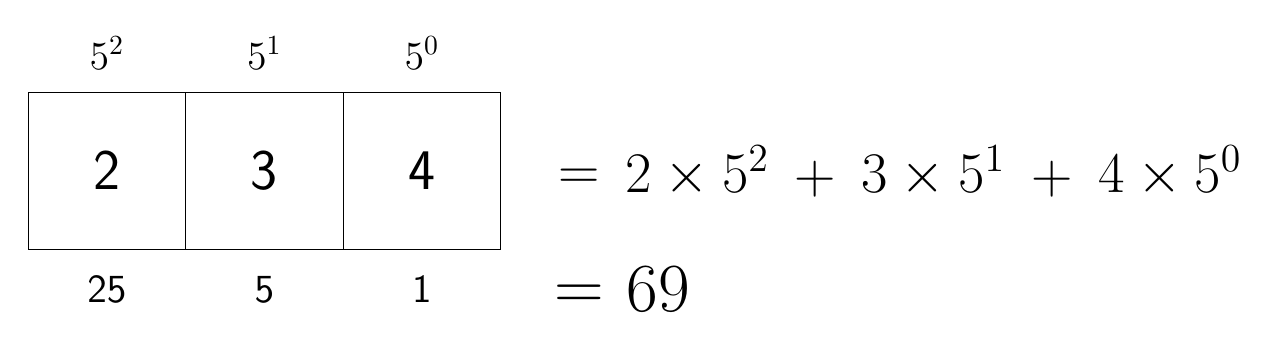
\begin{tikzpicture}
    \foreach \x/\y/\base/\dec in {0/2/2/25, 2/3/1/5, 4/4/0/1} {
        % Base value above the square
        \node at (\x,2.5) {\Large$5^{\base}$};
        % Draw the larger square
        \draw (\x-1,0) rectangle ++(2,2);
        % Number inside the square
        \node at (\x,1) {\huge \y};
        % Decimal value below the square
        \node at (\x,-0.5) {\Large\dec};
    }
    \node at (6,0.9) {\huge $=$};
    \node at (7.5,1) {\huge $2 \times 5^2$};
    \node at (9,0.9) {\huge $+$};
    \node at (10.5,1) {\huge $3 \times 5^1$};
    \node at (12,0.9) {\huge $+$};
    \node at (13.5,1) {\huge $4 \times 5^0$};

    \node at (6,-0.6) {\Huge $=$};
    \node at (7,-0.5) {\Huge $69$};
\end{tikzpicture}

\newpage
\subsection*{Self-assessment Questions from Foundation Maths Book}
\subsubsection*{Worked Example 14.2} Convert $83_{10}$ to binary.

\vspace*{0.5cm}

\noindent \textbf{Solution:}

\vspace*{0.25cm}

\noindent The general method for converting a decimal number to binary is to repeatedly divide the number by 2 and record the remainder. 
The binary number is then read from the remainders in reverse order.

\vspace*{0.25cm}

\noindent The steps for converting 83 to binary are as follows:

\begin{enumerate}
    \item $83 \div 2 = 41$ remainder 1
    \item $41 \div 2 = 20$ remainder 1
    \item $20 \div 2 = 10$ remainder 0
    \item $10 \div 2 = 5$ remainder 0
    \item $5 \div 2 = 2$ remainder 1
    \item $2 \div 2 = 1$ remainder 0
    \item $1 \div 2 = 0$ remainder 1
    \item The binary number is read from the remainders in reverse order: $1010011$
\end{enumerate}

\vspace*{0.5cm}

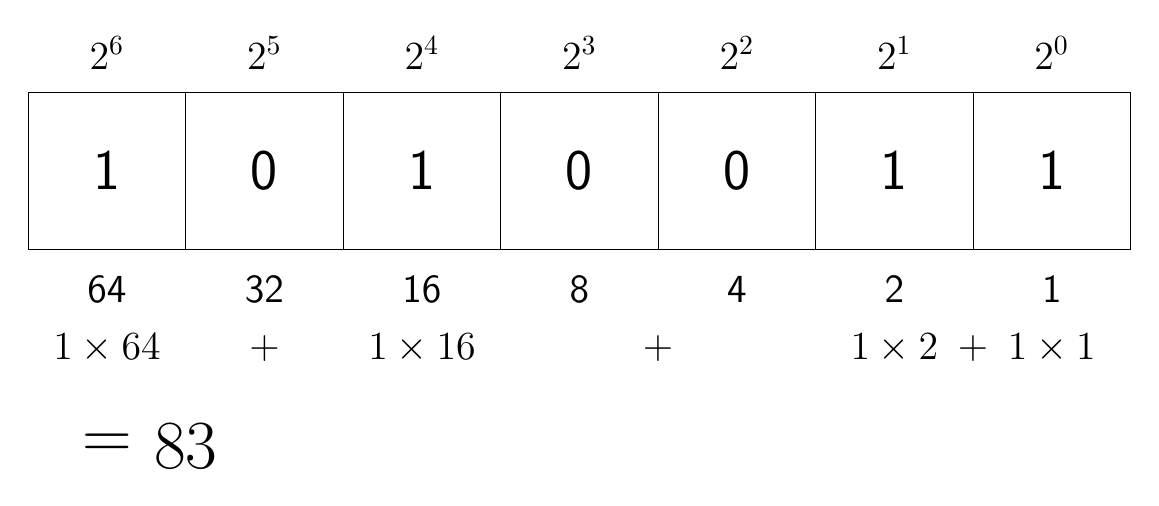
\begin{tikzpicture}
    \foreach \x/\y/\base/\dec in {0/1/6/64, 2/0/5/32, 4/1/4/16, 6/0/3/8, 8/0/2/4, 10/1/1/2, 12/1/0/1} {
        % Base value above the square
        \node at (\x,2.5) {\Large$2^{\base}$};
        % Draw the larger square
        \draw (\x-1,0) rectangle ++(2,2);
        % Number inside the square
        \node at (\x,1) {\huge \y};
        % Decimal value below the square
        \node at (\x,-0.5) {\Large\dec};
    }
    \node at (0,-1.25) {\Large $1 \times 64$};
    \node at (2,-1.25) {\Large $+$};
    \node at (4,-1.25) {\Large $1 \times 16$};
    \node at (7,-1.25) {\Large $+$};
    \node at (10,-1.25) {\Large $1 \times 2$};
    \node at (11,-1.25) {\Large $+$};
    \node at (12,-1.25) {\Large $1 \times 1$};

    \node at (0,-2.5) {\Huge $=$};
    \node at (1,-2.5) {\Huge $83$};

\end{tikzpicture}

\newpage

\subsubsection*{Exercise 14.2:} Convert the following decimal numbers to binary:
\vspace*{0.25cm}

\noindent (a): 19 (b): 36 (c): 100 (d): 796 (e): 5000

\vspace*{0.5cm}

\noindent \textbf{Solutions:}

\vspace*{0.25cm}

\noindent (a): $19_{10}$

\begin{enumerate}
    \item $19 \div 2 = 9$ remainder 1
    \item $9 \div 2 = 4$ remainder 1
    \item $4 \div 2 = 2$ remainder 0
    \item $2 \div 2 = 1$ remainder 0
    \item $1 \div 2 = 0$ remainder 1
    \item The binary number is read from the remainders in reverse order: $10011$
    \item $19_{10} = 10011_2$
    \item \textbf{Answer:} $19_{10} = 10011_2$
\end{enumerate}

\vspace*{0.5cm}

\noindent (b): $36_{10}$

\begin{enumerate}
    \item $36 \div 2 = 18$ remainder 0
    \item $18 \div 2 = 9$ remainder 0
    \item $9 \div 2 = 4$ remainder 1
    \item $4 \div 2 = 2$ remainder 0
    \item $2 \div 2 = 1$ remainder 0
    \item $1 \div 2 = 0$ remainder 1
    \item The binary number is read from the remainders in reverse order: $100100$
    \item $36_{10} = 100100_2$
    \item \textbf{Answer:} $36_{10} = 100100_2$
\end{enumerate}

\vspace*{0.5cm}

\noindent (c): $100_{10}$

\begin{enumerate}
    \item $100 \div 2 = 50$ remainder 0
    \item $50 \div 2 = 25$ remainder 0
    \item $25 \div 2 = 12$ remainder 1
    \item $12 \div 2 = 6$ remainder 0
    \item $6 \div 2 = 3$ remainder 0
    \item $3 \div 2 = 1$ remainder 1
    \item $1 \div 2 = 0$ remainder 1
    \item The binary number is read from the remainders in reverse order: $1100100$
    \item $100_{10} = 1100100_2$
    \item \textbf{Answer:} $100_{10} = 1100100_2$
\end{enumerate}

\vspace*{0.5cm}

\noindent (d): $796_{10}$

\begin{enumerate}
    \item $796 \div 2 = 398$ remainder 0
    \item $398 \div 2 = 199$ remainder 0
    \item $199 \div 2 = 99$ remainder 1
    \item $99 \div 2 = 49$ remainder 1
    \item $49 \div 2 = 24$ remainder 1
    \item $24 \div 2 = 12$ remainder 0
    \item $12 \div 2 = 6$ remainder 0
    \item $6 \div 2 = 3$ remainder 0
    \item $3 \div 2 = 1$ remainder 1
    \item $1 \div 2 = 0$ remainder 1
    \item The binary number is read from the remainders in reverse order: $1100011100$
    \item $796_{10} = 1100011100_2$
    \item \textbf{Answer:} $796_{10} = 1100011100_2$
\end{enumerate}

\vspace*{0.5cm}

\noindent (e): $5000_{10}$

\begin{enumerate}
    \item $5000 \div 2 = 2500$ remainder 0
    \item $2500 \div 2 = 1250$ remainder 0
    \item $1250 \div 2 = 625$ remainder 0
    \item $625 \div 2 = 312$ remainder 1
    \item $312 \div 2 = 156$ remainder 0
    \item $156 \div 2 = 78$ remainder 0
    \item $78 \div 2 = 39$ remainder 0
    \item $39 \div 2 = 19$ remainder 1
    \item $19 \div 2 = 9$ remainder 1
    \item $9 \div 2 = 4$ remainder 1
    \item $4 \div 2 = 2$ remainder 0
    \item $2 \div 2 = 1$ remainder 0
    \item $1 \div 2 = 0$ remainder 1
    \item The binary number is read from the remainders in reverse order: $1001110001000$
    \item $5000_{10} = 1001110001000_2$
    \item \textbf{Answer:} $5000_{10} = 1001110001000_2$
\end{enumerate}

\end{document}